% LTeX: language=en-US



\documentclass[draft,grl]{agutexSI2019}\usepackage[]{graphicx}\usepackage[]{xcolor}
% maxwidth is the original width if it is less than linewidth
% otherwise use linewidth (to make sure the graphics do not exceed the margin)
\makeatletter
\def\maxwidth{ %
  \ifdim\Gin@nat@width>\linewidth
    \linewidth
  \else
    \Gin@nat@width
  \fi
}
\makeatother

\definecolor{fgcolor}{rgb}{0.345, 0.345, 0.345}
\newcommand{\hlnum}[1]{\textcolor[rgb]{0.686,0.059,0.569}{#1}}%
\newcommand{\hlstr}[1]{\textcolor[rgb]{0.192,0.494,0.8}{#1}}%
\newcommand{\hlcom}[1]{\textcolor[rgb]{0.678,0.584,0.686}{\textit{#1}}}%
\newcommand{\hlopt}[1]{\textcolor[rgb]{0,0,0}{#1}}%
\newcommand{\hlstd}[1]{\textcolor[rgb]{0.345,0.345,0.345}{#1}}%
\newcommand{\hlkwa}[1]{\textcolor[rgb]{0.161,0.373,0.58}{\textbf{#1}}}%
\newcommand{\hlkwb}[1]{\textcolor[rgb]{0.69,0.353,0.396}{#1}}%
\newcommand{\hlkwc}[1]{\textcolor[rgb]{0.333,0.667,0.333}{#1}}%
\newcommand{\hlkwd}[1]{\textcolor[rgb]{0.737,0.353,0.396}{\textbf{#1}}}%
\let\hlipl\hlkwb

\usepackage{framed}
\makeatletter
\newenvironment{kframe}{%
 \def\at@end@of@kframe{}%
 \ifinner\ifhmode%
  \def\at@end@of@kframe{\end{minipage}}%
  \begin{minipage}{\columnwidth}%
 \fi\fi%
 \def\FrameCommand##1{\hskip\@totalleftmargin \hskip-\fboxsep
 \colorbox{shadecolor}{##1}\hskip-\fboxsep
     % There is no \\@totalrightmargin, so:
     \hskip-\linewidth \hskip-\@totalleftmargin \hskip\columnwidth}%
 \MakeFramed {\advance\hsize-\width
   \@totalleftmargin\z@ \linewidth\hsize
   \@setminipage}}%
 {\par\unskip\endMakeFramed%
 \at@end@of@kframe}
\makeatother

\definecolor{shadecolor}{rgb}{.97, .97, .97}
\definecolor{messagecolor}{rgb}{0, 0, 0}
\definecolor{warningcolor}{rgb}{1, 0, 1}
\definecolor{errorcolor}{rgb}{1, 0, 0}
\newenvironment{knitrout}{}{} % an empty environment to be redefined in TeX

\usepackage{alltt}

\usepackage{graphicx}
\usepackage{booktabs}
\setkeys{Gin}{draft=false} % Allow figure display.

\usepackage{color}
\newcommand*{\todo}[1]{\textbf{\textcolor{red}{(#1)}}}

\authorrunninghead{RAUPACH AND ALDRIDGE}
\titlerunninghead{CHANGES IN DAMAGING HAIL IN AUSTRALIA}

\authoraddr{Corresponding author: T. H. Raupach,
UNSW Sydney Climate Change Research Centre,
Mathews Building Level 4, 
UNSW Sydney, 
New South Wales 2052,
Australia
(timothy.h.raupach@gmail.com)}
\IfFileExists{upquote.sty}{\usepackage{upquote}}{}
\begin{document}

\title{Supporting Information for ``Changes in damaging hail in major Australian cities with global warming''}
% % %DOI: 10.1002/%insert paper number here%

\authors{Timothy H. Raupach\affil{1,2,3}, Joanna Aldridge\affil{4,5}}

\affiliation{1}{UNSW Institute for Climate Risk and Response, 
                UNSW Sydney, New South Wales, Australia}
\affiliation{2}{UNSW Climate Change Research Centre, 
                UNSW Sydney, New South Wales,  Australia}
\affiliation{3}{ARC Centre of Excellence for Climate Extremes, 
                Sydney, New South Wales,  Australia}
\affiliation{4}{School of Geosciences, University of Sydney, 
                Sydney, New South Wales,  Australia}
\affiliation{5}{QBE Australia, Sydney, 
                New South Wales, Australia}

\begin{article}

\noindent\textbf{Contents of this file}
\begin{enumerate}
    \item Description of recent high-loss hail events in Australia.
    \item Figures S1 to S8.
    \item Tables S1 to S4.
\end{enumerate}

\clearpage

\section*{Description of recent high-loss hail events in Australia}

\subsection*{``Hailoween''}

The 31 October 2020 ``Hailoween'' hail storm generated a series of at least nine
supercells in a corridor from Amberley to Logan, Queensland \cite<unless
otherwise noted, details here are sourced from>{AIDR_2021}. The cells generated
giant hail stones reported as 7 cm in Gympie, up to 14 cm at Forestdale, 13 cm
at Hillcrest, 9.5 cm at Amberley, 8 cm at Springfield, 7 cm at Gatton, and 5 cm
at Seventeen Mile Rocks. The hardest hit suburbs were Springfield, Springfield
Lakes, Rosewood, and Willowbank. Strong winds were also recorded, with 100 km
h$^{-1}$ gusts occurring around Moreton Bay, and wind damage evident from
Redcliffe to Kingston. The State Emergency Service received over 2,900 callouts
and power outages affected 95,000 homes. The storms were associated with a
series of complex fronts and embedded lows in the monsoon inland trough,
following a week of instability over eastern Australia \cite{BOM_2020,
BOM_2024}. The Queensland Reconstruction Authority (QRA)’s initial assessment
found 520 severely damaged properties, 602 moderately damaged properties and 652
properties with minor damage \cite{Ipswich_2021}. Extensive damage was reported
to roofs, skylights, solar panels, interiors, awnings, windows, shutters,
including ceiling collapse and fallen trees (pers. comm. J. Aldridge 2024).
Water ingress following hail damage was widespread, leading to damage to
interior walls and floors, mold, and contents damage (pers. comm. J. Aldridge
2024). Some houses experienced hail damage through the roof and interior ceiling
and into the living areas of the home \cite{ABC_2020b}. This event resulted in
an insured loss of \$A1.056b from around 44,700 claims \cite{ICA_2024}.

\subsection*{Tri-city storms}

The 18-20th January 2020 ``tri-city'' storms impacted a wide area of eastern
Australia immediately following the devastating ``Black Summer'' bushfires
\cite<unless otherwise noted, details here are sourced from the>{AIDR_2020}. The
storms impacted three major cities: Canberra, Sydney, and Melbourne, as well as
country New South Wales areas of Queanbeyan and Goulburn \cite{ICA_2024}.
Canberra received 4--6 cm hail which impacted the central business district and
densely populated inner suburbs including the Australian National University. A
117 km h$^{-1}$ wind gust was recorded at Canberra Airport. The extensive damage
in Canberra included broken windows and skylights in homes and commercial
buildings, flooding, and thousands of cars damaged by hailstones. Wind damage
included fallen trees, branches and power lines, and blocked roads. There was
damage to buildings at the Australian National University and in the central
business district \cite{ABC_2020c}. Melbourne received hail of up to 5.5 cm over
the southeastern suburbs, and there were damaging winds, heavy rainfall and
flash flooding across broader regions. Sydney received large hail over the outer
southern suburbs around Campbelltown \cite{ABC_2020d}. The meteorological
situation showed an inland trough extending from central Queensland through
southeastern Australia, with an upper level low and associated surface level low
creating moist unstable air \cite{BOM_2024}. In total, this event resulted in
around 132,000 claims and a \$A1.68b insured loss \cite{ICA_2024}.

\subsection*{Rockhampton hailstorm}

The 19 April 2020 hailstorm \cite{ABC_2020, EWN_2020, Swissre_2021} impacted the
central Queensland towns of Rockhampton and Yeppoon and surrounding areas
\cite{ABC_2020} located near the Tropic of Capricorn. The weather pattern was
due to an upper-level trough crossing central Queensland, combined with a
surface trough \cite{EWN_2020}. Storm activity propagated from inland moving
northeast to the coast \cite{EWN_2020}, with a large supercell impacting the
corridor from Rockhampton to Yeppoon. Giant hail of up to 12 cm was reported
\cite{EWN_2020}, as well as 100 km h$^{-1}$ wind gusts \cite{ABC_2020}. Damage
included holes in roofs, smashed windows and car windscreens, and tree damage
\cite{ABC_2020}. The timing of this event during the first Covid lockdown
complicated recovery efforts \cite{AFR_2020}. An insured loss of \$A503m from
around 15,000 claims was incurred \cite{ICA_2024}. In the Whitsunday region,
golf ball size hail was reported in Sarina \cite{EWN_2020}. The time of year,
size of hail and the tropical latitude of this event made it highly unusual.

\begin{figure}[!h]
    \includegraphics[width=\textwidth]{figures/domains}
    \caption{Approximate extents of the model domains on a map of Australia. The
    coarse-resolution ($\sim$27 km grid spacing) domains are in yellow,
    medium-resolution ($\sim$9 km grid spacing) domains in dark green, and
    fine-resolution ($\sim$3 km grid spacing) domains in blue. The solid and
    dotted lines group the two sets of nested domains that were calculated
    together. Approximate city locations (with city extents not shown) are
    marked with red points for Perth (a), Kalgoorlie (b), Adelaide (c),
    Melbourne (d), Canberra (e), Sydney (f), and Brisbane (g). Note that two
    model configurations were used, with settings other than the domain
    configurations the same for both.}
    \label{fig:domains}
\end{figure}

\begin{figure}[!ht]
    \centering
    \includegraphics[width=0.9\textwidth]{figures/maxes_Adelaide_hailcast_diam_max}
    \includegraphics[width=0.9\textwidth]{figures/maxes_Brisbane_hailcast_diam_max}
    \includegraphics[width=0.9\textwidth]{figures/maxes_Kalgoorlie_hailcast_diam_max}
    \includegraphics[width=0.9\textwidth]{figures/maxes_Melbourne_hailcast_diam_max}
    \includegraphics[width=0.9\textwidth]{figures/maxes_Perth_hailcast_diam_max}
    \includegraphics[width=0.9\textwidth]{figures/maxes_Sydney_Canberra_hailcast_diam_max}
    \caption{Maximum hail size diameters for the Adelaide, Brisbane, Kalgoorlie,
    Melbourne, Perth, and Sydney/Canberra domains under the historical and
    future scenarios, with and without ocean areas removed. Subsetting to land
    used the WRF land mask with small holes filled and a slight erosion applied
    so that points over the ocean, large bodies of water, or directly over the
    coastal boundary are not considered in this study.}
    \label{fig:maxes_with_removed_pts}
\end{figure}

\begin{figure}[!ht]
    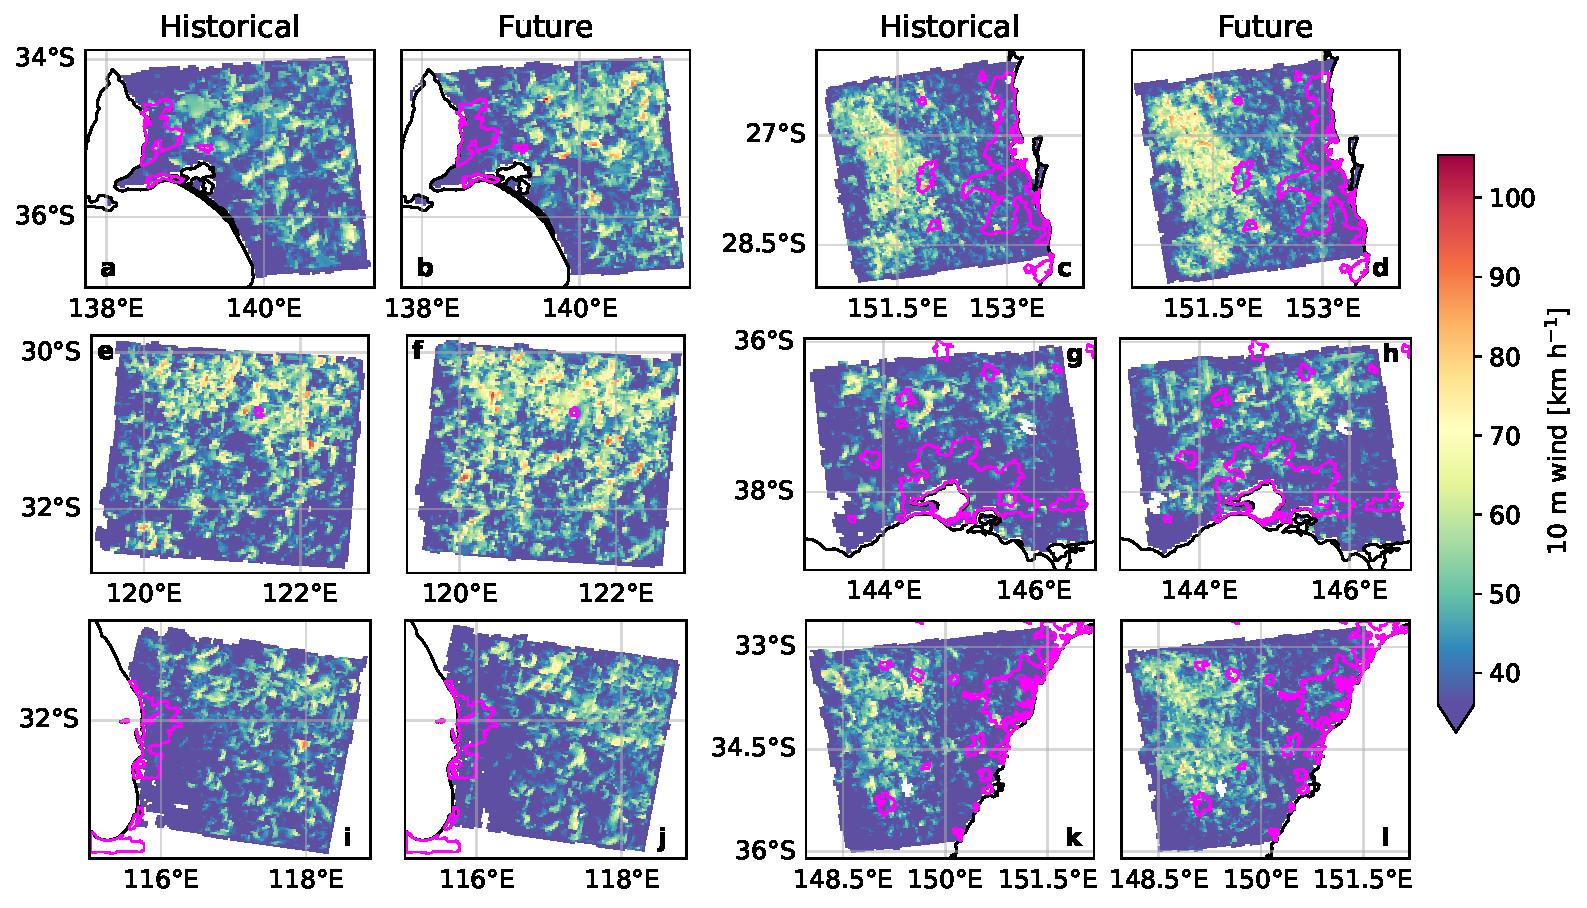
\includegraphics[width=\textwidth]{figures/max_10m_winds_by_domain}
    \caption{Maximum 10 m wind speed at hail times in historical and future climates, for Adelaide (a, b), Brisbane (c, d), Kalgoorlie (e, f), Melbourne (g, h), Perth (i, j) and Sydney/Canberra (k, l) domains. Fuchsia outlines show significant urban areas \cite{ABS_2022}. To increase contrast, the color scale is truncated.}
    \label{fig:max_wind_by_domain}
\end{figure}

\begin{figure}[!ht]
    \includegraphics[width=\textwidth]{figures/timeseries_hail}
    \caption{Time series of daily maximum hail sizes by domain and epoch. Gaps exist because only the convective season was simulated each year.}
    \label{fig:timeseries_hail}
\end{figure}

\begin{figure}[!ht]
    \includegraphics[width=\textwidth]{figures/timeseries_wind}
    \caption{As for Figure \ref{fig:timeseries_hail}, but for daily maximum 10 m wind collocated with hail.}
    \label{fig:timeseries_wind}
\end{figure}

\begin{figure}[!ht]
    \includegraphics[width=\textwidth]{figures/gev_dists_hail}
    \caption{Densities of maximum daily hail size per domain and epoch derived from WRF simulations and the fitted EVD (Generalized Pareto with 20 mm threshold) models.}
    \label{fig:densities_hail}
\end{figure}

\begin{figure}[!ht]
    \includegraphics[width=\textwidth]{figures/gev_dists_wind}
    \caption{As for Figure \ref{fig:densities_hail}, but for daily maximum 10 m wind collocated with hail fitted with Generalized Extreme Value models.}
    \label{fig:densities_wind}
\end{figure}

\begin{figure}[!ht]
    \includegraphics[width=\textwidth]{figures/qq_hail}
    \caption{Quantile-quantile plots for EVD models fitted to daily maximum hail sizes, per domain and epoch.}
    \label{fig:qq_hail}
\end{figure}

\begin{figure}[!ht]
    \includegraphics[width=\textwidth]{figures/qq_wind}
    \caption{Quantile-quantile plots for EVD models fitted to daily maximum 10 m wind collocated with hail.}
    \label{fig:qq_wind}
\end{figure}

\begin{figure}[!ht]
    \includegraphics[width=\textwidth]{figures/fit_pvals}
    \caption{Distributions of $p$ values from KS tests, comparing WRF
     values to EVD models, and historical EVDs to future EVDs, per variable and
     domain. For each test, the KS test was applied 100 times with 1000 random
     values drawn from the relevant EVD(s) each time, to obtain a
     distribution of $p$ values. Bars show medians, box hinges show the
     interquartile ranges (IQRs), whiskers show the largest (smallest) values no
     more than 1.5 $\times$ IQR from the upper (lower) hinge, and points show
     outlier points beyond the whisker ranges. The red horizontal line shows $p
     = 0.05$; when $p$ values are below this line the null hypothesis that the
     two samples come from the same distribution can be rejected.}
    \label{fig:ks_pvals}
\end{figure}

\begin{figure}[!ht]
    \includegraphics[width=\textwidth]{figures/fit_params}
    \caption{Location (a, d), scale (b, e), and shape (c, f) parameters for
    fitted EVD distributions for maximum hail size (a--c) and 10 m wind at
    hail hours (d--f). Parameter values are shown as a point and whiskers show
    95\% confidence intervals.}
    \label{fig:evd_parameters}
\end{figure}

\begin{figure}[!ht]
    \includegraphics[width=\textwidth]{figures/correlations}
    \caption{Correlations of seasonal values of hail-relevant properties
    between domains, by epoch. Seasonal means were calculated from daily means
    at hail locations and hours. Variables considered are seasonal hail days
    (a, g), and mean hail diameter (b, h), 10 m wind at hail hours (c, i),
    bulk vertical wind shear (d, j), CAPE (e, k), lifted index (f, l), CIN (m,
    r), 700-500 hPa lapse rate (n, s), temperature at 500 hPa (o, t), freezing
    level height (p, u) and melting level height (q, v), for historical (a-f,
    m-q) and future (g-l, r-v) epochs. Statistically significant correlations
    are shown by an $\ast{}$ for 90\% confidence level ($p <$ 0.1),
    $\ast{}\!\ast{}$ for 95\% confidence level ($p <$ 0.05), and
    $\ast{}\!\ast{}\!\!\ast{}$ for the 99\% confidence level ($p <$ 0.01).}
    \label{fig:correlations}
\end{figure}

\begin{table}
    \centering
    \caption{Probability of a hail day exceeding hail sizes of 50 or 100 mm, and of coincident wind exceeding 80 and 100 km h$^{-1}$, per domain and epoch.}
    \label{tab:exceedence_probs}
    \begin{tabular}{llcccc}
    \hline
    & & \multicolumn{2}{c}{Hail probability [\%]} & \multicolumn{2}{c}{Wind probability [\%]} \\ 
    Domain & Epoch & 50 mm & 100 mm & 80 km h$^{-1}$ & \multicolumn{1}{c}{100 km h$^{-1}$} \\ 
    \hline
Adelaide & Historical  & $21.96$ & $\phantom{0}4.44$ & $\phantom{0}1.70$ & $\phantom{0}0.00$ \\ & Future  & $22.89$ & $\phantom{0}4.07$ & $\phantom{0}5.40$ & $\phantom{0}1.00$ \\Brisbane & Historical  & $21.94$ & $\phantom{0}2.04$ & $\phantom{0}1.63$ & $\phantom{0}0.02$ \\ & Future  & $21.25$ & $\phantom{0}2.27$ & $\phantom{0}2.06$ & $\phantom{0}0.01$ \\Kalgoorlie & Historical  & $11.96$ & $\phantom{0}0.52$ & $\phantom{0}9.02$ & $\phantom{0}0.00$ \\ & Future  & $21.40$ & $\phantom{0}1.64$ & $13.01$ & $\phantom{0}0.23$ \\Melbourne & Historical  & $\phantom{0}9.08$ & $\phantom{0}0.42$ & $\phantom{0}1.26$ & $\phantom{0}0.05$ \\ & Future  & $24.23$ & $\phantom{0}2.64$ & $\phantom{0}0.59$ & $\phantom{0}0.00$ \\Perth & Historical  & $14.49$ & $\phantom{0}0.58$ & $\phantom{0}1.84$ & $\phantom{0}0.00$ \\ & Future  & $20.52$ & $\phantom{0}0.00$ & $\phantom{0}0.89$ & $\phantom{0}0.00$ \\Sydney/Canberra & Historical  & $14.22$ & $\phantom{0}1.28$ & $\phantom{0}0.57$ & $\phantom{0}0.01$ \\ & Future  & $18.17$ & $\phantom{0}1.40$ & $\phantom{0}0.24$ & $\phantom{0}0.00$ \\
    \hline 
    \end{tabular}
\end{table}

\begin{table}[!ht]
    \caption{Parameterization schemes used in the WRF simulations.}
    \label{tab:schemes}
    \centering
    \begin{tabular}{lr}
          \hline
          Microphysics & P3-3moment \cite{Milbrandt_JAS_2021} \\
          Cumulus (medium and coarse nests only) & New Tiedtke \cite{Zhang_JC_2017} \\
          Long wave and shortwave radiation & RRTMG \cite{Iacono_JGRA_2008} \\
          Planetary boundary layer & YSU \cite{Hong_MWR_2006} \\
          Surface layer & Revised MM5 \cite{Jimenez_MWR_2012} \\
          Land surface & Noah-MP \cite{Niu_JGRA_2011} \\
          \hline
    \end{tabular}
\end{table}

\begin{table}[!ht]
    \centering
    \caption{Mean $\pm$ standard deviation of seasonal hail days in historic
    and future simulations, and relative future change with 95\% confidence
    interval, per domain. Statistical significance is indicated by $\ast{}$
    for a 90\% confidence level ($p < 0.1$) and $\ast{}\!\ast{}$ for a 95\%
    confidence level ($p < 0.05$).}
    \label{tab:frequency}  
    \begin{tabular}{lrrr@{}l@{}r}
          \hline
          Domain & Historic days & Future days & \multicolumn{3}{r}{Future change} \\ 
          \hline
Adelaide  & 8.7 $\pm$ 4.2 & 8.35 $\pm$ 4.9 & -4\% & $$ & (-38\% to 30\%) \\Brisbane  & 32.95 $\pm$ 8.3 & 37.8 $\pm$ 8.8 & 15\% & $\,\ast{}$ & (-2\% to 31\%) \\Kalgoorlie  & 10 $\pm$ 6 & 9.8 $\pm$ 5.2 & -2\% & $$ & (-38\% to 34\%) \\Melbourne  & 11.7 $\pm$ 5.9 & 11.5 $\pm$ 7.1 & -2\% & $$ & (-37\% to 34\%) \\Perth  & 6.8 $\pm$ 4.9 & 7.55 $\pm$ 4.9 & 11\% & $$ & (-35\% to 57\%) \\Sydney/Canberra  & 24.3 $\pm$ 9.4 & 31.4 $\pm$ 9 & 29\% & $\,\ast{}\!\ast{}$ & (5\% to 53\%) \\
          \hline 
     \end{tabular}
\end{table}

\begin{table} 
    \centering
    \caption{Mean values in the historical epoch, at hail times, by domain.
    Averages are on daily values except for hail days which are seasonal.
    Variables are convective available potential energy (CAPE, in J kg$^{-1}$),
    convective inhibition (CIN, in J kg$^{-1}$), freezing level height (FLH, in
    m), hail size (in mm), lifted index (LI, in K), lapse rate between 700 hPa
    and 500 hPa (LR, in K km$^{-1}$), melting level height (MLH, in m), bulk
    vertical wind shear between 0 and 6 km (S06, in m s$^{-1}$), temperature at
    500 hPa (T500, in K), and 10 m wind (Wind, in m s$^{-1}$).}
    \label{tab:hist_means}
    \begin{tabular}{lcccccc}
        \hline
        Variable  & Adelaide & Brisbane & Kalgoorlie & Melbourne & Perth & \multicolumn{1}{c}{Sydney/Canberra} \\ 
        \hline        
Hail days  & $\phantom{000}\phantom{-}8.7$ & $\phantom{00}\phantom{-}33.0$ & $\phantom{00}\phantom{-}10.0$ & $\phantom{00}\phantom{-}11.7$ & $\phantom{000}\phantom{-}6.8$ & $\phantom{00}\phantom{-}24.3$ \\Mean wind  & $\phantom{00}\phantom{-}18.4$ & $\phantom{00}\phantom{-}16.5$ & $\phantom{00}\phantom{-}20.5$ & $\phantom{00}\phantom{-}15.0$ & $\phantom{00}\phantom{-}18.4$ & $\phantom{00}\phantom{-}14.7$ \\Max wind  & $\phantom{00}\phantom{-}44.1$ & $\phantom{00}\phantom{-}43.5$ & $\phantom{00}\phantom{-}55.5$ & $\phantom{00}\phantom{-}38.9$ & $\phantom{00}\phantom{-}43.9$ & $\phantom{00}\phantom{-}37.7$ \\MLH  & $\phantom{-}3837.1$ & $\phantom{-}4050.7$ & $\phantom{-}4192.2$ & $\phantom{-}3737.3$ & $\phantom{-}4154.6$ & $\phantom{-}3844.9$ \\Mean hail  & $\phantom{00}\phantom{-}12.6$ & $\phantom{00}\phantom{-}13.9$ & $\phantom{00}\phantom{-}12.3$ & $\phantom{00}\phantom{-}12.8$ & $\phantom{00}\phantom{-}12.5$ & $\phantom{00}\phantom{-}12.4$ \\S06  & $\phantom{00}\phantom{-}19.6$ & $\phantom{00}\phantom{-}15.8$ & $\phantom{00}\phantom{-}18.4$ & $\phantom{00}\phantom{-}18.2$ & $\phantom{00}\phantom{-}17.0$ & $\phantom{00}\phantom{-}16.7$ \\CAPE  & $\phantom{0}\phantom{-}255.3$ & $\phantom{0}\phantom{-}460.1$ & $\phantom{0}\phantom{-}255.8$ & $\phantom{0}\phantom{-}300.6$ & $\phantom{0}\phantom{-}317.4$ & $\phantom{0}\phantom{-}317.5$ \\LI  & $\phantom{000}\phantom{-}0.8$ & $\phantom{000}-1.6$ & $\phantom{000}-0.6$ & $\phantom{000}-0.7$ & $\phantom{000}-0.7$ & $\phantom{000}-0.8$ \\CIN  & $\phantom{00}-97.6$ & $\phantom{0}-121.5$ & $\phantom{0}-143.4$ & $\phantom{00}-96.8$ & $\phantom{0}-125.9$ & $\phantom{0}-103.5$ \\LR  & $\phantom{000}-6.5$ & $\phantom{000}-6.2$ & $\phantom{000}-6.6$ & $\phantom{000}-6.4$ & $\phantom{000}-6.5$ & $\phantom{000}-6.5$ \\T500  & $\phantom{0}\phantom{-}261.5$ & $\phantom{0}\phantom{-}263.2$ & $\phantom{0}\phantom{-}263.5$ & $\phantom{0}\phantom{-}261.1$ & $\phantom{0}\phantom{-}263.4$ & $\phantom{0}\phantom{-}261.6$ \\FLH  & $\phantom{-}3931.4$ & $\phantom{-}4162.6$ & $\phantom{-}4293.2$ & $\phantom{-}3827.6$ & $\phantom{-}4261.9$ & $\phantom{-}3946.3$ \\Max hail  & $\phantom{00}\phantom{-}28.8$ & $\phantom{00}\phantom{-}31.5$ & $\phantom{00}\phantom{-}23.7$ & $\phantom{00}\phantom{-}23.0$ & $\phantom{00}\phantom{-}23.7$ & $\phantom{00}\phantom{-}24.8$ \\
    \hline 
    \end{tabular}
\end{table}

\begin{table}
    \centering
    \caption{Radar-based hail statistics per domain for convective seasons
    (October-February) only. Calculated using Bureau of Meteorology radar data
    \cite{Soderholm_radar_data}. Columns show the approximate percentage of the
    model domain covered by radar data (\% cover), the percentage of overall
    hail days containing Maximum Expected Size of Hail
    \cite<MESH,>{Witt_WF_1998} over 50 mm (50 mm) and 100 mm (100 mm), the
    resulting return period in years on 100 mm (RP 100 mm) and 50 mm (RP 50 mm)
    hail, and the mean number of seasonal hail days defined as days with MESH
    over 21 mm per season (Hail days). Radar data was processed as in
    \citeA{Raupach_npjCAS_2023} and aggregated to maximum MESH value per
    0.25\deg{} x 0.25\deg{} grid cell. We note that radars have different
    sampling periods per site, radar instruments have changed over time
    \cite<e.g.>{Warren_QJRMS_2020}, and that MESH values are subject to
    uncertainty \cite<e.g.>{Greco_WF_2024}.}
    \label{tab:radar_stats}
    \begin{tabular}{lrrrrrr}
        Domain & \% cover & 50 mm & 100 mm & RP 100 mm & RP 50 mm & Hail days \\
        \hline
Adelaide & 90.5 & 17.9 & 0.5 & 25.0 & 1.8 & 7.6 \\Brisbane & 93.8 & 35.1 & 0.0 & -- & 1.0 & 43.4 \\Kalgoorlie & 81.5 & 20.1 & 0.0 & -- & 1.1 & 11.9 \\Melbourne & 95.7 & 22.5 & 0.0 & -- & 1.1 & 17.6 \\Perth & 89.7 & 18.2 & 0.0 & -- & 1.9 & 8.4 \\Sydney/Canberra & 96.6 & 30.4 & 0.1 & 28.0 & 1.2 & 45.2 \\
    \end{tabular}
\end{table}

\bibliography{../main/library}
\end{article}

\end{document}
